\subsection{Søgemodul}
\label{sub:s_searchmodul}

Søgemodulet implementerer en sorteringsfunktion, som muliggør søgning på både og brugere.

\begin{figure}
  \centering
  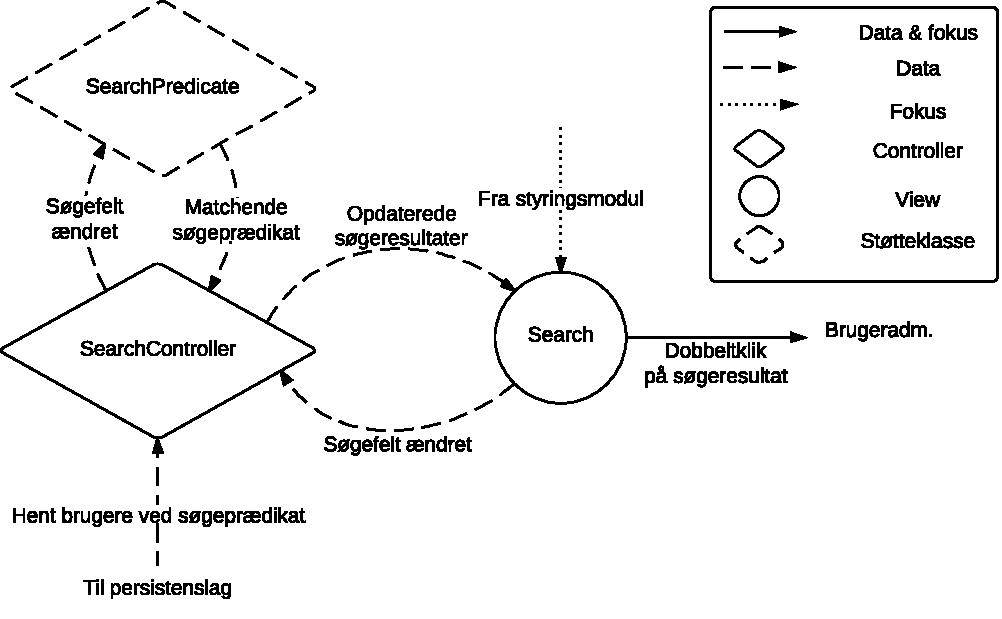
\includegraphics[width=\textwidth]{search-diagram.pdf}
  \caption{Dette er bare noget filler tekst.}
\end{figure}
\subsubsection{Funktionalitet}
\label{sub:funktionalitet}

Søgemodulets funktion er at sortere en liste af medlemmer og gæster, ud fra brugerdefinerede kriterier. Der kan sorteres efter alle datafelter som en bruger kan have. Derudover er det muligt at sortere efter datafelter som en brugers båd eller rejser indeholder. 

\subsubsection{Implementation}
\label{sub:implementation}

Søgemodulet består af et Search-element, et SearchPredicate og en SearchController. Search-elementet tager brugerens individuelle inputs/kriterier og sender dem til SearchControlleren. SearchControlleren sender dataen til SearchPredicate som der sender et prædikat tilbage. SearchControlleren sammenligner prædikatet med persistenslaget der derefter sender \quote{hits} tilbage til SearchControlleren. SearchControlleren sender \quote{hits}'ne tilbage til Search-elementet der viser resultaterne i det respektive felt. Dette køre hvergang der kommer et nyt input i form af et tegn, hvilket gør at resultaterne bliver opdateret ved hvert tasteklik


% subsection implementation (end)

% subsection funktionalitet (end)

% subsection s_gemodul (end)
